\section{Background and The Initialization Anomaly}
\label{sec:background}

\subsection{Cauer-Topology RC Thermal Networks}

State-of-the-art architectural simulators approximate heat transfer using equivalent electrical RC circuits based on the well-established Cauer topology. In this duality, electrical current ($I$) represents power dissipation ($P$ in Watts), voltage ($V$) represents temperature ($T$ in Kelvin or Celsius), electrical resistance ($R$) corresponds to thermal resistance (\si{\kelvin\per\watt}), and electrical capacitance ($C$) represents thermal capacitance or thermal mass (\si{\joule\per\kelvin}).

A minimal, computationally efficient thermal model commonly used for rapid architectural DTM evaluation is the two-node lumped-parameter model (representing the silicon die and the chip package). The state space of such a system is governed by a system of first-order ordinary differential equations (ODEs):
\begin{align}
    C_{die} \frac{dT_{die}}{dt} &= P_{in} - \frac{T_{die} - T_{pkg}}{R_{die}} \label{eq:tdie} \\
    C_{pkg} \frac{dT_{pkg}}{dt} &= \frac{T_{die} - T_{pkg}}{R_{die}} - \frac{T_{pkg} - T_{amb}}{R_{pkg}} \label{eq:tpkg}
\end{align}
where $T_{amb}$ denotes the fixed ambient boundary condition. Simulators typically solve these ODEs numerically using explicit methods (e.g., Forward Euler) or implicit methods (e.g., Backward Euler or Runge-Kutta).

\begin{figure}[t]
\centering
% 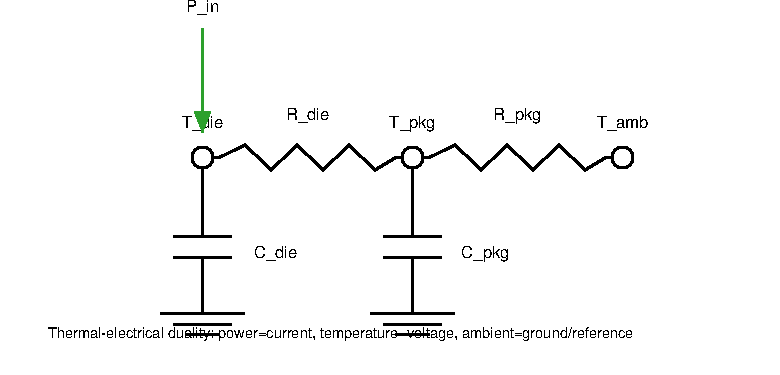
\includegraphics[width=0.8\linewidth]{figures/cauer_topology.pdf}
\caption{Equivalent electrical RC circuit for the two-node Cauer thermal model (Die and Package).}
\label{fig:cauer_topology}
\end{figure}

\subsection{The Absolute-Zero Initialization Artifact in gem5}

For a thermal simulation to yield physically admissible transient results, the initial state vector $\mathbf{T}(t=0)$ must reflect a valid thermodynamic equilibrium or a defined physical state. Typically, assuming the chip starts from a cold state, all node temperatures should initialize to the ambient temperature:
\begin{equation}
    T_{die}(0) = T_{pkg}(0) = T_{amb}
\end{equation}

However, source code analysis of the gem5 simulator's \texttt{ThermalModel} implementation reveals a severe initialization artifact. While the primary ambient node is correctly populated, intermediate nodes within the RC network (such as the package or heatsink nodes) are instantiated via default C++ constructors without explicit temperature assignments. Consequently, their initial state defaults to exactly \SI{0}{\kelvin} (absolute zero).

\subsection{Mathematical Consequence on Transient Dynamics}

To understand the severity of this artifact, consider the first discrete numerical integration step using the Forward Euler method with a time step $\Delta t$. Substituting $T_{pkg}(0) = \SI{0}{\kelvin}$ into the discretized form of Eq.~\ref{eq:tdie}:
\begin{equation}
    T_{die}(\Delta t) \approx T_{amb} + \frac{\Delta t}{C_{die}} \left( P_{in} - \frac{T_{amb} - 0}{R_{die}} \right)
\end{equation}

Because $T_{amb}$ is typically around \SI{298}{\kelvin} (\SI{25}{\degreeCelsius}), the term $\frac{T_{amb} - 0}{R_{die}}$ acts as an artificial, massive heat sink. Even under maximum processor power dissipation ($P_{in}$), this spurious gradient dominates the right-hand side of the equation. 
Physically, this simulates the die instantaneously dumping its thermal energy into a surrounding medium that is at absolute zero. The result is a precipitous, non-monotonic drop in the die junction temperature during the initial simulation epochs. 

Recent literature highlights that transient stability and monotonic warm-up are critical for evaluating DTM controllers \cite{fasttherm2024}. A scheduler observing this artificial cooling might prematurely boost the CPU frequency, entirely corrupting the resulting performance/thermal co-simulation trace.
